\documentclass{beamer}

% === AUTOR === (((
\author{\textit{Por Erick I. Rodríguez Juárez.}}
% )))

% === PAQUETES === (((
% \usepackage{makeidx}
% \usepackage{xltxtra}
\usepackage{amsfonts}
\usepackage{amsmath}
\usepackage{amssymb}
% \usepackage{fullpage}
\usepackage{tikz}
\usetikzlibrary{arrows.meta}
\usepackage{graphicx}
% )))

% === TIPOGRAFÍA === (((
% \setmainfont[
  % BoldFont       = bodonibi,
	% ItalicFont     = Century modern italic2.ttf,
	% BoldItalicFont = bodonibi,
	% SmallCapsFont  = lmromancaps10-regular.otf
% ]{Century_modern.ttf}
% )))

% === COMANDOS === (((
% \newcommand{\dis}{\displaystyle}
% \newcommand{\qed}{\hspace{0.5cm}\rule{0.16cm}{0.4cm}}
% \newcommand{\operator}[1]{\mathop{\vphantom{\sum}\mathchoice
% {\vcenter{\hbox{\huge $#1$}}}
% {\vcenter{\hbox{\Large $#1$}}}{#1}{#1}}\displaylimits}
% \newcommand{\suma}{\operator{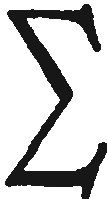
\includegraphics[scale=0.09]{FOTOS/Sigma.png}}}
% \setlength{\parindent}{0mm}
% )))

% === ITALICA EN ENTORNO MATEMÁTICO === (((
% \DeclareSymbolFont{italics}{\encodingdefault}{\rmdefault}{m}{it}
% \DeclareSymbolFontAlphabet{\mathit}{italics}
% \ExplSyntaxOn
% \int_step_inline:nnnn { `A } { 1 } { `Z }
 % {  \exp_args:Nf \DeclareMathSymbol{\char_generate:nn{#1}{11}}{\mathalpha}{italics}{#1} }
% \int_step_inline:nnnn { `a } { 1 } { `z } {  \exp_args:Nf \DeclareMathSymbol{\char_generate:nn{#1}{11}}{\mathalpha}{italics}{#1}}
% \ExplSyntaxOff
% )))

\begin{document}

\frame{\titlepage}

\section{E.D. No Homogéneas.} % (((
\begin{frame}[t]
	\frametitle{E.D. No Homogéneas.}
	\begin{block}{}
		Recordemos que una E.D. No Homogénea tiene la forma
		\[
			a_m(x) y^{(n)}+a_{m-1} y^{(n-1)} + \;\cdots\; + a_1(x) y' + a_0(x) y = g(x) .
		\]
		donde \(a_i(x)\) y \(g(x)\) son funciones continuas en \(I\), y \(a_n(x) \ne 0\), \(\forall x \in I\).
	\end{block}
	\begin{block}{Solución de la E.D.N.H.}
		Sea \(y_p(x)\) cualquier solución paricular de la E.D. No Homogénea de orden \(n\) en el intervalo \(I\). Sea \(y_c(x)\) la solución general de la E.D.H asociada a la E.D. en \(I\), llamada \textit{función complementaria}. Entonces la solución general de la E.D. No Homogénea en el intervalo \(I\), es:
		\[
			y(x) = y_c(x) + y_p(x).
		\]
		Es decir:
	\end{block}
\end{frame}

\begin{frame}[t]
	\begin{block}{}
		\[
			y(x) +c_1y_1(x) + \;\cdots\; + c_ny_n(x) + y_p(x).
		\]
		\(c_1, \;\ldots,\; c_n\) son ocnstantes arbitrarias, donde \(y_1,y_2, \;\ldots,\; y_n\) es un c.f.s de la E.D.L.H asociada. \\[2mm]
		Para determinar la solución particular de una E.D. No Homogénea estudiaremos dos métodos:
		\begin{enumerate}
			\item Método de coeficientes indeterminados.
			\item Método de variación de parámetros.
		\end{enumerate}
	\end{block}
\end{frame}
% )))

\section{Método de Coef. Indeterminados.} % (((
\begin{frame}[t]
	\frametitle{Método de Coeficientes Indeterminados.}
	\begin{block}{}
		La idea básica de éste método es proponer la forma de \(y_p(x)\)de acuerdo a los tipos de funciones que forman a \(g(x)\), donde \(g(x)\) puede ser: constante, función polinomial, función exponencial, función seno y/o cosenos, sumas y/o productos finitos de éstas funciones. \\[2mm]
		Para ilustrar el método considere los siguientes eventos.
	\end{block}
	\begin{example}
		Determine la solución general de la E.D. \(y'' + 2y' -3y=g(x)\), donde
		\begin{enumerate}
			\item \(g(x) = 8e^{2x}\).
			\item \(g(x) = (x-1) ^2\).
			\item \(g(x) = 7 \cos 3x\).
		\end{enumerate}
	\end{example}
\end{frame}
\begin{frame}[t]
\end{frame}

\begin{frame}[t]
	\begin{block}{Excepción.}
		El método de Coeficientes Indeterminados falla cuando \(g(x)\) es solución de la Ecuación Diferencial Homogéna asociada.
	\end{block}
	\begin{example}
		Suponga que \(g(x) =e^{-3x}\) en el ejemplo anterior, luego, encuentre una solución particular de la E.D.N.H.
		\[
			y'' +2y' -3y=e^{-3x}.
		\]
	\end{example}
\end{frame}
\begin{frame}[t]
\end{frame}

\begin{frame}[t]
	\begin{alertblock}{Ejercicio.}
		Obtener la solución del P.V.I. \(y'' +4y' +4y=(3+x) e^{-2x}\), con
		\[
			y(0) = 2 \;,\; y' (0) =5.
		\]
	\end{alertblock}
\end{frame}

\begin{frame}[t]
	\begin{block}{}
		Sean \(y_1,y_2, \;\ldots,\; y_k\) soluciones particulares de una E.D.N.H con \(g_1, g_2, \;\ldots,\; g_k\), respectivamente. Esto es, \(y_i\) representa la solución particular de la E.D. \(a_n(x) y^(n) + a_{n-1} (x) y^{(n-1)} + \;\cdots\; + a_1(x) y' +a_0y = g_i(x)\), entonces
		\[
			\;\implies\; y(x) = y_1+ y_2+ \;\cdots\; +y_k(x),
		\]
		es solución paicular de la E.D.N.H.
		\[
			a_n(x) y^{(n)} + a_{n-1} y^{(n-1)} + \;\cdots\; + a_1(x) y' +a_0y=g_1(x) + \;\cdots\; g_k(x).
		\]
	\end{block}
	\begin{example}
		Obtener la solución general de la E.D.N.H siguiente:
		\[
			y''' -4y' = 2x+5-e^{-2x}.
		\]
	\end{example}
\end{frame}
% )))

\section{Método de Variación de Parámetros.} % (((
\begin{frame}[t]
	\frametitle{Método de Variación de Parámetros.}
	\begin{block}{}
		Consideremos la E.D.L.N.H. de segundo orden en su forma estándar,
		\[
			y'' + P(x) y' +Q(x) y = G(x)
		\]
		Luego, el método de variación de parámetros
		\[
			y_p(x) = \mu _1(x) y_1(x) + \mu _2(x) y_2(x)
		\]
		donde \(\{y_1,y_2\}\) conforman un conjunto fundamental de soluciones de la E.D. Homogńea asociada.
		\[
			y(x) = c_1y_1 + c_2y_2.
		\]
		Así pues, sustituyendo \(y_p\), \(yp'\), \(yp''\), en la E.D. y después de factorizar de manera conveniente, se encuentra que \(\mu _1(x)\) y \(\mu _2(x)\) deben satisfacer las siguientes ecuaciones
	\end{block}
\end{frame}

\begin{frame}[t]
	\begin{block}{}
		\[
			\begin{array}{rcl}
				y_1(x) \mu _1' (x) +y_2(x) \mu _2' (x) & = & 0 \\[2mm]
				y_1' (x) \mu _1' (x) + y_2'(x) \mu _2' (x) & = & G(x) .
			\end{array}
		\]
		Usamos la regla de Cramer para resolver este sistema.
		\[
			\begin{array}{rcl}
				\mu_1 '(x) & = & \dfrac{\begin{vmatrix}
					0 & y_2(x) \\
					G(x) & y_2'(x)
				\end{vmatrix}}{\begin{vmatrix}
					y_1(x) & y_2(x) \\
					y_1' (x) & y_2' (x)
				\end{vmatrix}} = \dfrac{-y_2(x) G(x)}{W[y_1,y_2] (x)} \\[1cm]
				\mu_2 '(x) & = & \dfrac{\begin{vmatrix}
					y_1(x) & 0 \\
					y_1'(x) & G(x)
				\end{vmatrix}}{\begin{vmatrix}
					y_1(x) & y_2(x) \\
					y_1' (x) & y_2' (x)
				\end{vmatrix}} = \dfrac{y_1(x) G(x)}{W[y_1,y_2] (x)}
			\end{array}
		\]
		Luego, integramos con respecto a \(x\),
	\end{block}
\end{frame}

\begin{frame}[t]
	\begin{block}{}
		\[
			\mu _1(x) = \dis\int \dfrac{-y_2(x) G(x)}{W[y_1,y_2] (x)} dx \hspace{5mm} y \hspace{5mm} \mu _2(x) = \dis\int \dfrac{y_1(x) G(x)}{W[y_1,y_2] (x)} dx.
		\]
		Por consiguiente,
		\[
			y_p(x) = \bigg(\dis\int \dfrac{-y_2(x) G(x)}{W[y_1,y_2] (x)} dx\bigg) y_1(x) + \bigg(\dis\int \dfrac{y_1(x) G(x)}{W[y_1,y_2] (x)} dx\bigg) y_2(x).
		\]
	\end{block}
	\begin{example}
		Considere la E.D. \(y'' +y = \tan x\). Encuentre la solución general de la E.D.
	\end{example}
\end{frame}
\begin{frame}[t]
\end{frame}

\begin{frame}[t]
	\begin{alertblock}{Ejercicio.}
		Resuelve el P.V.I. \(y'' -4y' +4y=(12x^2-6x) e^{2x}\), con \(y(0) =1\), \(y' (0) =1\). Use el método de variación de parámetros para encontrar una solución particular de la E.D.N.H.
	\end{alertblock}
\end{frame}
\begin{frame}[t]
\end{frame}

\begin{frame}[t]
	\begin{example}
		Discuta, como se pueden utilizar los métodos de coeficientes indeterminados y el de variación de parámetros para resolver la E.D.
		\[
			y'' -2y' +y = 4x^2-3+x^{-1} e^x.
		\]
	\end{example}
\end{frame}
% )))

\section{Método de Variación de Parámetros para E.D. de Orden \(n\).} % (((
\begin{frame}[t]
	\begin{block}{}
		\frametitle{Método de Variación de Parámetros para E.D. de Orden \(n\).}
		El método de variación de parámetros se puede generalizar para E.D.L. de Orden \(n\), de la forma
		\[
			y^{(n)} + p_{n-1} (x) y^{(n-1)} + \;\cdots\; +p_1(x) y' + p_0(x) y = G(x).
		\]
		Si:
		\[
			y_c(x) = c_1y_1(x) + c_2y_2(x) + \;\cdots\; + c_ny_n(x).
		\]
		es la solución genral de la E.D.H asociada, entonces, se propone como solución particular
		\[
			y_p(x) = \mu _1(x) y_1(x) + \;\cdots\; \mu _ny_n(x),
		\]
		donde \(\mu _i(x)\), \(i=1, \;\ldots,\; n\), están determinadas por el siguiente sistema de ecuaciones:e
	\end{block}
\end{frame}

\begin{frame}[t]
	\begin{block}{}
		\vspace{-5mm}
			\begin{align*}
				y_1 \mu ' _1            &+          y_2 \mu ' _2            &+     \;\cdots\;    &+     y_n \mu _n'           &=    0 \\
				y_1' \mu ' _1           &+          y_2' \mu ' _2           &+     \;\cdots\;    &+     y_n' \mu _n'          &=    0 \\
				& & & &\vdots \\
				y_1^{(n-1)} \mu ' _1    &+          y_2^{(n-1)} \mu ' _2    &+     \;\cdots\;    &+     y_n^{(n-1)} \mu _n'   &=    0
			\end{align*}
			La solución del sistema se obtiene con regla de Cramer
			\[
				\mu _i' = \dfrac{W_i}{W}, \hspace{5mm} i=1,2, \;\ldots,\; n
			\]
			\(W =\) Wronskiano de \(y_1, y_2, \;\ldots,\; y_n\), \\[2mm]
			\(W_i=\) es el determinante de la matriz de coeficientes por el vector del lado derecho del sistema. \\[2mm]
			Luego, \(\mu _i\) se obtiene integrando con respecto a \(x\).
	\end{block}
\end{frame}

\begin{frame}[t]
	\begin{example}
		Resueve por variación de parámetros la siguiente E.D.N.H \(y''' +4y' = \sec 2x\).
	\end{example}
\end{frame}
% )))

\end{document}
